% !Tex program = pdflatex
% =====================================================================
%  Template de rapport — Laboratoire de développement logiciel
%  Compilation : pdflatex -> bibtex -> pdflatex -> pdflatex
%  (sous Emacs/AUCTeX : C-c C-c LaTeX, puis BibTeX, puis LaTeX x2)
%
%  Author: Vincent ENGLEBERT
%  Révisions
%  28/10/2026: création du template
% =====================================================================
\documentclass[a4paper,11pt]{article}

% --------------------------- Encodage & langue -----------------------

\usepackage[utf8]{inputenc}
\usepackage[T1]{fontenc}
\usepackage[sfdefault]{atkinson}   % Atkinson comme police sans-serif PAR DÉFAUT\usepackage{natbib}
\usepackage[french]{babel}
\usepackage[a4paper,margin=2.5cm]{geometry}

% --------------------------- Packages --------------------------------
\usepackage{graphicx}
\usepackage{booktabs}
\usepackage{enumitem}
\usepackage{xcolor}
\usepackage{pgfgantt}
\usepackage{hyperref}
\usepackage{natbib}
\usepackage{csquotes}
\usepackage{comment}
\usepackage{graphicx}   % préambule



\hypersetup{colorlinks=true, linkcolor=blue!50!black,
            urlcolor=blue!50!black, citecolor=blue!50!black}
\setlength{\parindent}{0pt}
\setlength{\parskip}{0.6em}

\newcommand{\coursnom}{Projet Individuel INFOB318}



% =====================================================================
%  INFORMATIONS À COMPLÉTER (page de garde)
% =====================================================================

\newcommand{\anneeacad}{2026--2027}
\newcommand{\projetcode}{CODE-PROJET}
\newcommand{\projetnom}{Nom du projet}
\newcommand{\etudiantnom}{TALON}
\newcommand{\etudiantprenoms}{Achille Gustave}
\newcommand{\matricule}{007007}


% =====================================================================
\begin{document}

% --------------------------- PAGE DE GARDE ---------------------------
\begin{titlepage}
  \centering
  \vspace*{1.5cm}
  {\large \coursnom\par}
  {\large Année académique \anneeacad\par}
  \vspace{3cm}
  {\Large\bfseries\scshape Projet \projetcode\par}
  \vspace{0.8cm}
  {\Huge\bfseries \projetnom\par}
  \vfill
  \begin{tabular}{rl}
    \textbf{Étudiant(e)} & \etudiantnom{} \etudiantprenoms \\[0.4em]
    \textbf{Matricule}   & \matricule
  \end{tabular}
  \vspace{2cm}
  \par
  {\today}
\end{titlepage}


\clearpage\newpage


\section*{Préambule}

Modifiez les informations sous le commentaire
\begin{verbatim}
% ===========================================
%  INFORMATIONS À COMPLÉTER (page de garde)
%  ===========================================
\end{verbatim}
afin de produire une page de garde personnalisée.

Pensez à nettoyer le document de toutes les directives qui y sont
énoncées afin de ne garder que les informations propres à votre
projet.

\section{Liste des fonctionnalités}
\label{sec:fonctionnalites}

Listez ici la liste des fonctionnalités attendues de votre logiciel en
suivant les modèles ci-dessous.

\begin{itemize}

\item En tant que [rôle], je veux [action], afin de [bénéfice métier].

\item En tant que [rôle], je veux pouvoir [résultat], afin de [valeur].

\item Quand [contexte], je veux [besoin], afin de [résultat attendu].

\item En tant que [rôle], je peux [action], sous réserve de [règle], afin de [objectif].

\item En tant que [rôle], je veux que [règle métier] soit appliquée lors de [événement], afin de [objectif].

\end{itemize}

Exemples concrets pour chaque modèle à propos d'un éditeur de texte en ligne.

\begin{enumerate}

\item[F001] En tant qu'utilisateur, je veux pouvoir sauvegarder les
  versions de mon document, afin de ne pas perdre d'informations en
  cas d'erreurs.

\item[F002] En tant qu'administrateur, je veux pouvoir bloquer un
  compte rapidement, afin de sécuriser les accès.

\item[F003] Quand un utilisateur a travaillé plus de 10 minutes, je veux une
  sauvegarde automatique, afin de ne pas perdre d'informations.

\item[F004] En tant qu'administrateur, je peux désactiver le serveur
  applicatif, sous réserve que toutes les modifications aient été
  sauvegardées, afin de faire une maintenance.

\item[F005] En tant qu'administrateur, je veux que tous les documents
  soient sauvegardés lors d'une désactivation, afin de ne perdre
  aucune information.

\end{enumerate}


\section{Liste des qualités}
\label{sec:qualites}

Exigences non fonctionnelles du projet (par exemple selon ISO/IEC~25010 :
performance, fiabilité, sécurité, maintenabilité, utilisabilité, portabilité\ldots).

\begin{enumerate}
\item[Q001] L'application se conformera aux règles du WCGA $\geq 2.2$.
\item[Q002] Les communications entre le client et le serveur seront chiffrées.
\item[Q003] Le serveur sera déployable sans connaissances techniques de docker.
\end{enumerate}

\clearpage\newpage
\section{Modèle ERA du domaine d'application}
\label{sec:era}

Modèle entité-relation des informations utiles pour la réalisation de
votre projet. Ce modèle n'est pas celui de la base de données: il est
plus large et sert de référence pour définir la terminologie et les
liens sémantiques entre les termes. Si votre projet comporte une base
de données, alors cette dernière sera modélisée par un autre modèle
ERA aligné sur le premier. On peut définir ce modèle comme une sorte
de pense-bête de tous les concepts utiles à votre réflexion.

Attention, le modèle doit être produit avec DB-MAIN. Il garantit que
le modèle est bien formé syntaxiquement.

% includegraphics (Menu "copy graphics" dans DB-MAIN)
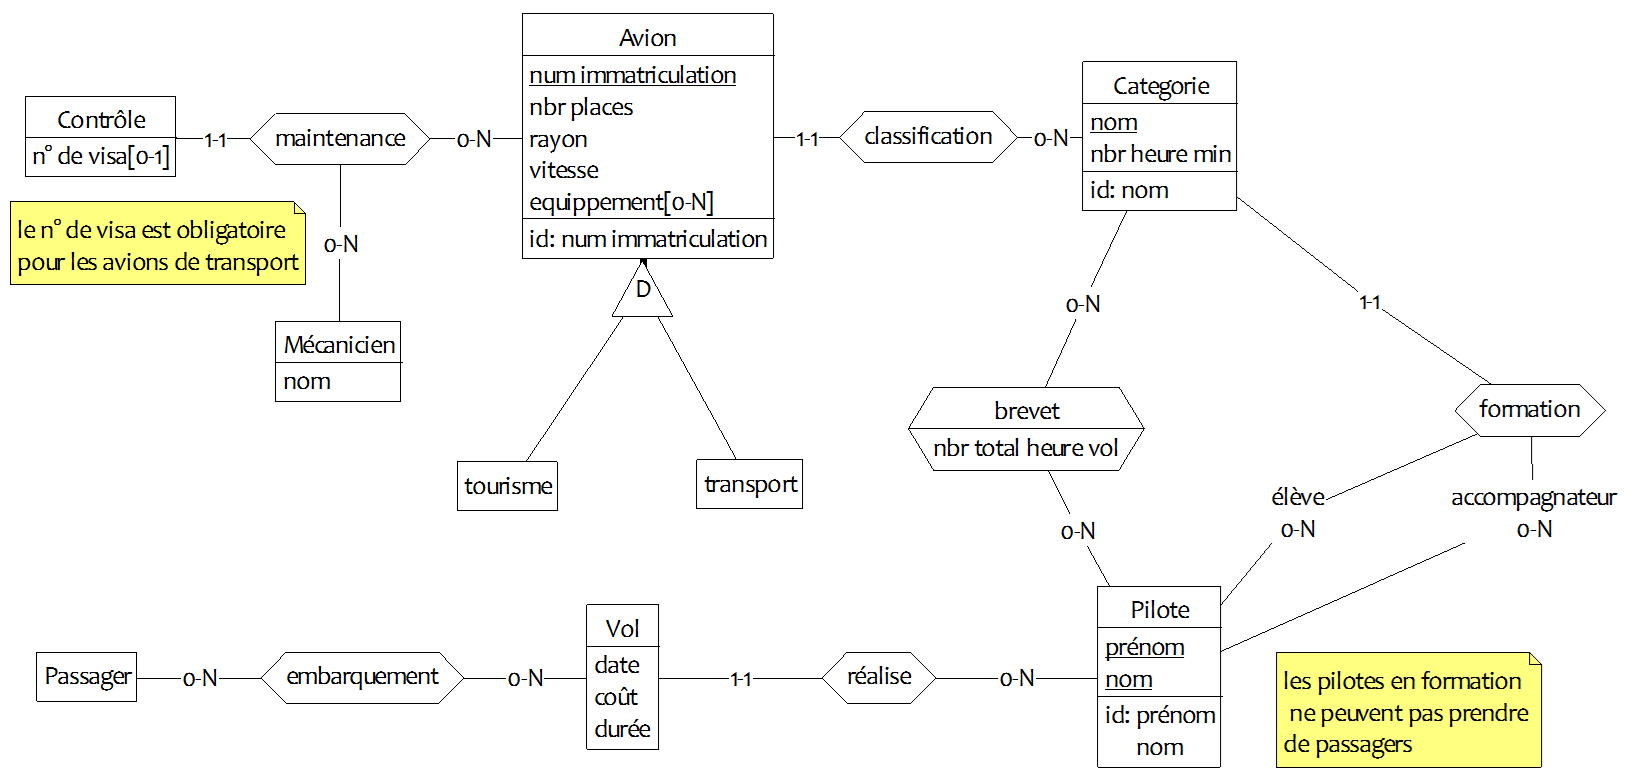
\includegraphics[width=\linewidth]{era}


\clearpage\newpage
\section{Diagramme de Gantt}
\label{sec:gantt}



% includegraphics (Gantt de la feuille Excel)
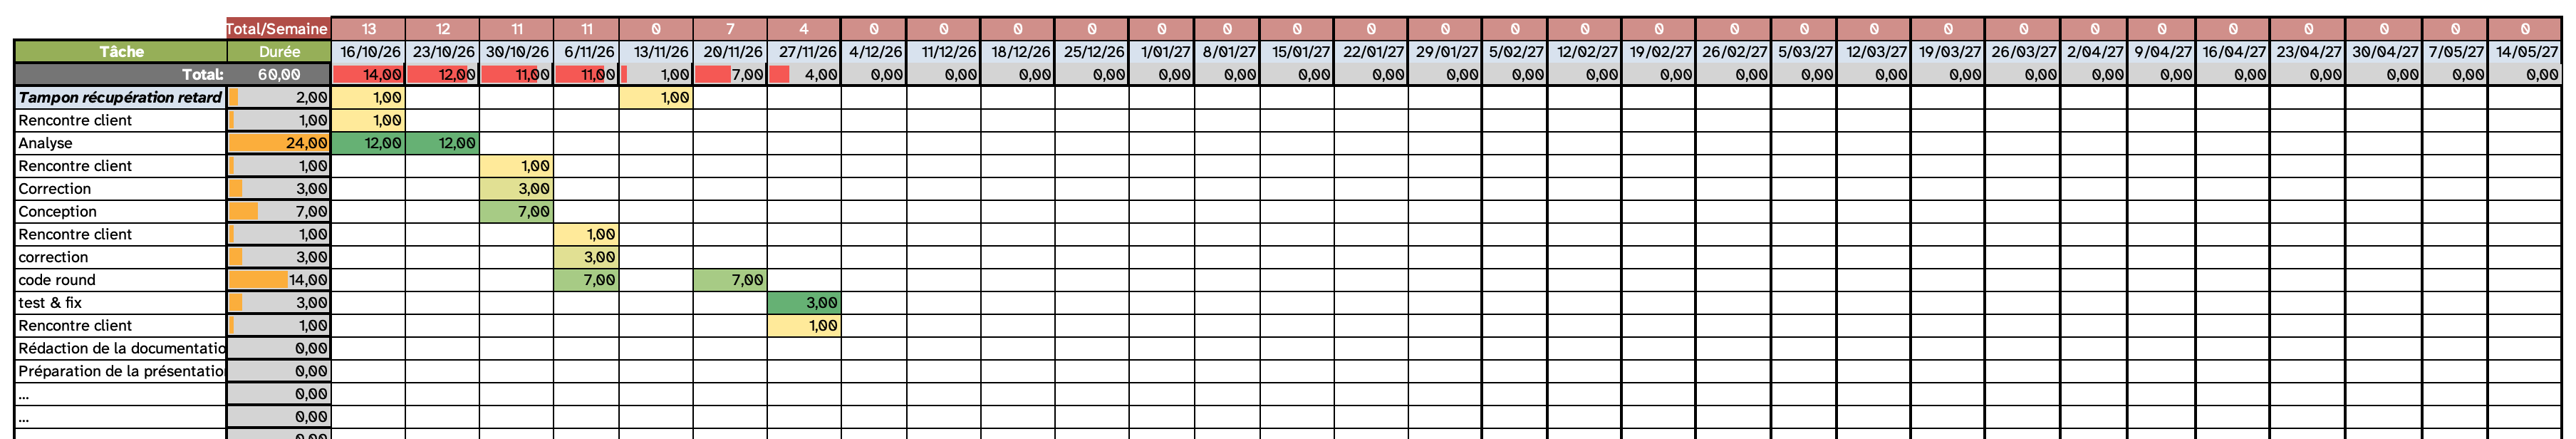
\includegraphics[width=\linewidth]{gantt}


\section{Sources d'informations consultées}
\label{sec:sources}

\nocite{*} % retirer pour n'afficher que les références citées avec \cite{}
\bibliographystyle{plain}
\bibliography{references}

\subsection*{Autres sources (non BibTeX)}
\begin{itemize}
  \item Documentation, sites web, cours, échanges avec l'encadrant\ldots
\end{itemize}

\section{Remarques}
\label{sec:remarques}



\end{document}
